\documentclass{standalone}
\usepackage{tikz}
\usetikzlibrary{patterns, positioning}
\usepackage[sfdefault]{ClearSans} %% option 'sfdefault' activates Clear Sans as the default text font
\usepackage[T1]{fontenc}

\begin{document}
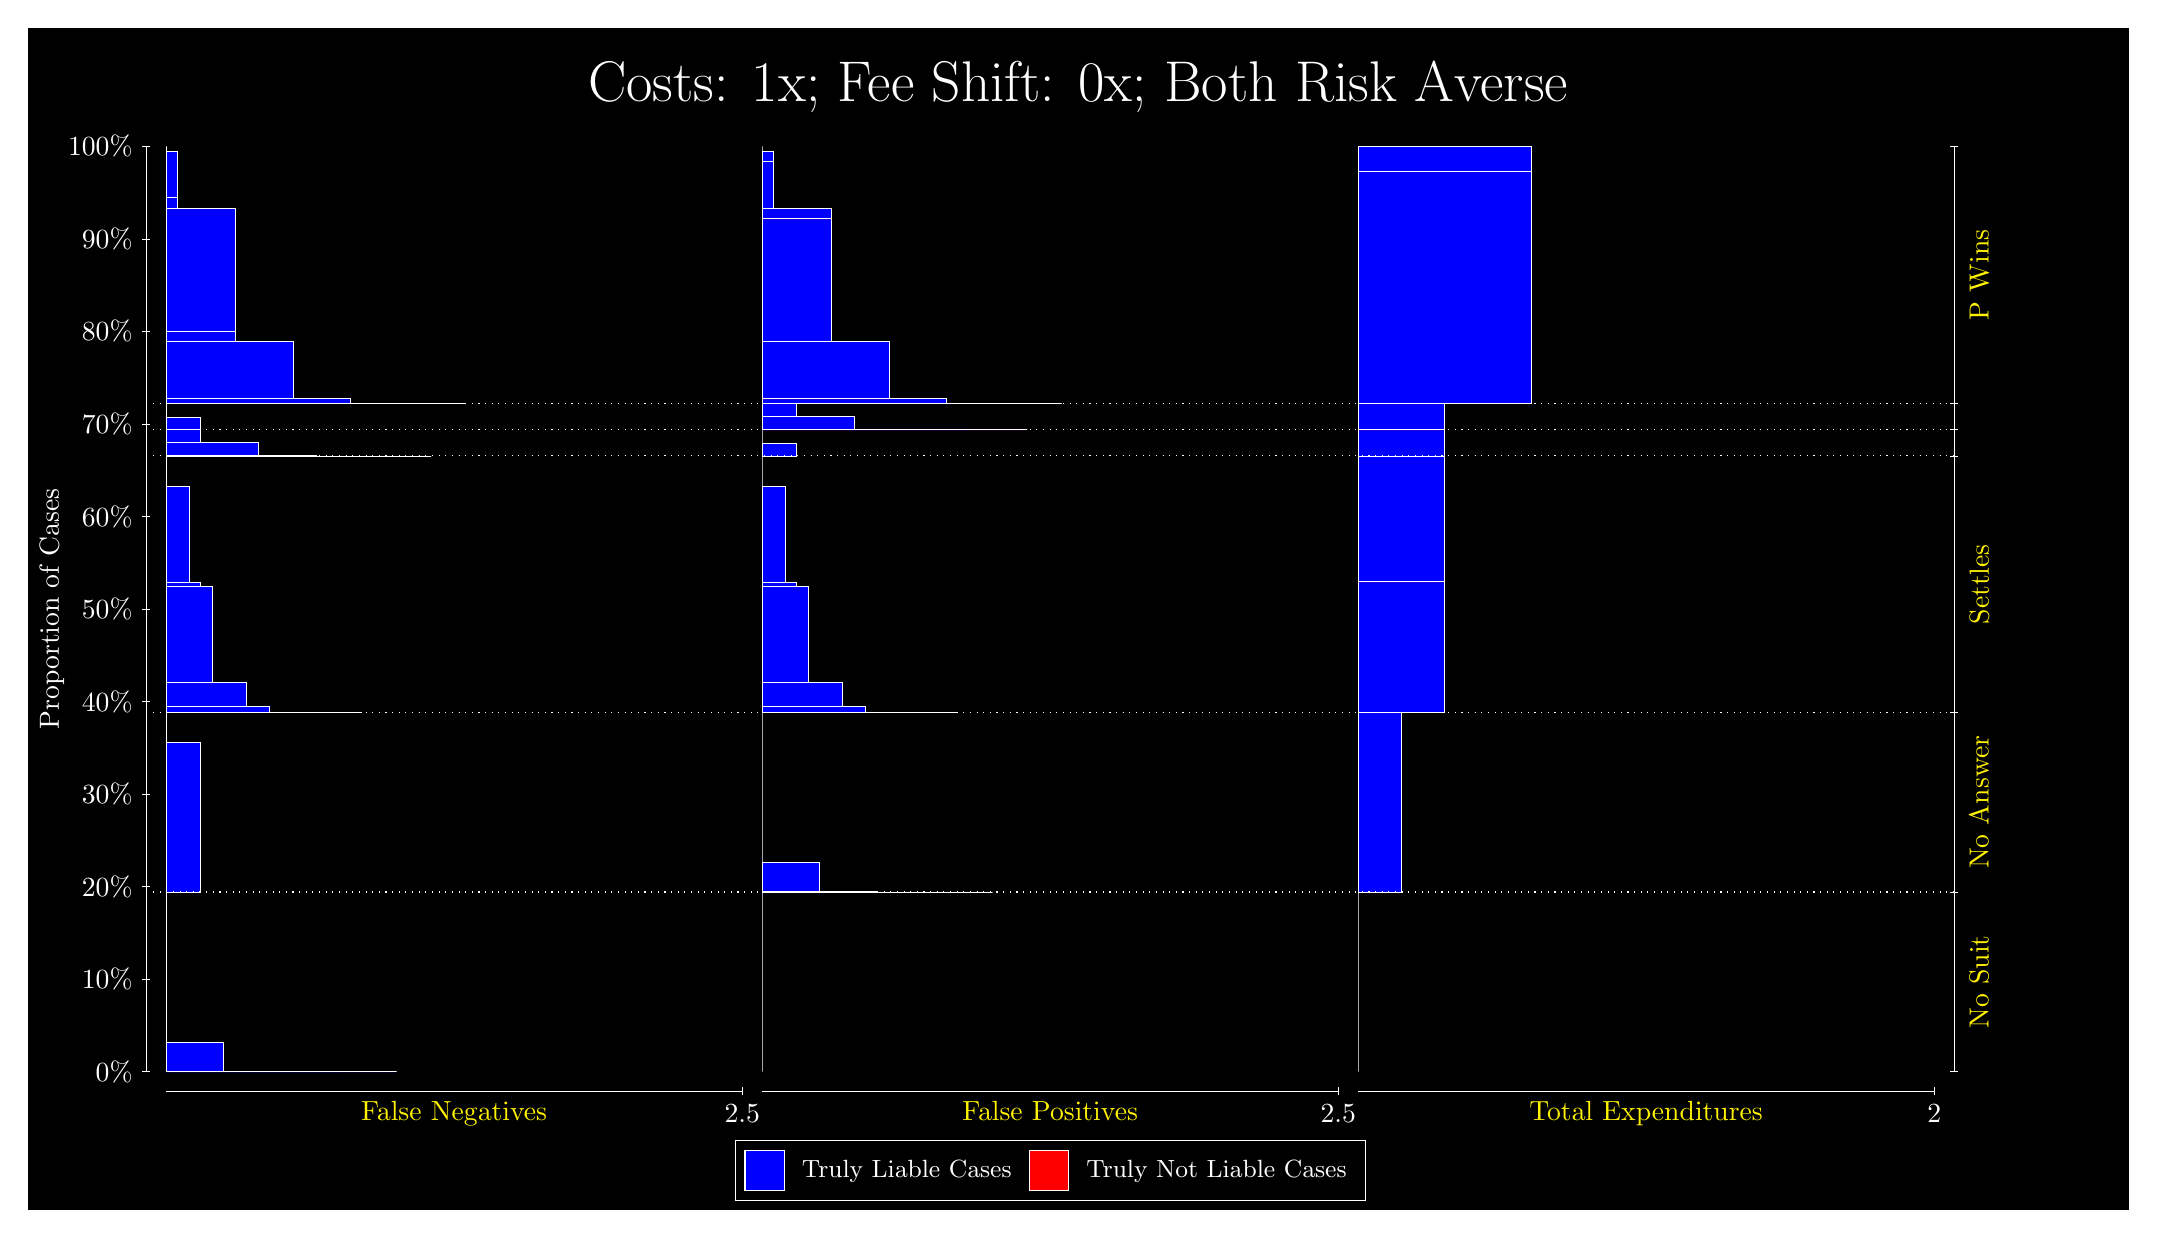
\begin{tikzpicture}
\draw[fill=black] (0,0) rectangle (26.667,15);
\draw[text=white] (0,13.5) rectangle (26.667,15) node[midway] {\huge Costs: 1x; Fee Shift: 0x; Both Risk Averse};
\draw[white, very thin] (1.5,1.75) -- (1.5,13.5);
\node[rotate=90, text=white, anchor=center] at (0.3, 7.625) {Proportion of Cases};
\draw[white, very thin] (1.45,1.75) -- (1.55,1.75);
\node[text=white, anchor=east] at (1.45, 1.75) {0\%};
\draw[white, very thin] (1.45,2.925) -- (1.55,2.925);
\node[text=white, anchor=east] at (1.45, 2.925) {10\%};
\draw[white, very thin] (1.45,4.1) -- (1.55,4.1);
\node[text=white, anchor=east] at (1.45, 4.1) {20\%};
\draw[white, very thin] (1.45,5.275) -- (1.55,5.275);
\node[text=white, anchor=east] at (1.45, 5.275) {30\%};
\draw[white, very thin] (1.45,6.45) -- (1.55,6.45);
\node[text=white, anchor=east] at (1.45, 6.45) {40\%};
\draw[white, very thin] (1.45,7.625) -- (1.55,7.625);
\node[text=white, anchor=east] at (1.45, 7.625) {50\%};
\draw[white, very thin] (1.45,8.8) -- (1.55,8.8);
\node[text=white, anchor=east] at (1.45, 8.8) {60\%};
\draw[white, very thin] (1.45,9.975) -- (1.55,9.975);
\node[text=white, anchor=east] at (1.45, 9.975) {70\%};
\draw[white, very thin] (1.45,11.15) -- (1.55,11.15);
\node[text=white, anchor=east] at (1.45, 11.15) {80\%};
\draw[white, very thin] (1.45,12.325) -- (1.55,12.325);
\node[text=white, anchor=east] at (1.45, 12.325) {90\%};
\draw[white, very thin] (1.45,13.5) -- (1.55,13.5);
\node[text=white, anchor=east] at (1.45, 13.5) {100\%};

\draw[white, very thin] (24.457,1.75) -- (24.457,13.5);
\draw[white, very thin] (24.407,1.75) -- (24.507,1.75);
\node[anchor=west] at (24.407, 1.75) {};
\draw[white, very thin] (24.407,4.0302) -- (24.507,4.0302);
\node[anchor=west] at (24.407, 4.0302) {};
\draw[white, very thin] (24.407,6.3104) -- (24.507,6.3104);
\node[anchor=west] at (24.407, 6.3104) {};
\draw[white, very thin] (24.407,9.568) -- (24.507,9.568);
\node[anchor=west] at (24.407, 9.568) {};
\draw[white, very thin] (24.407,9.9023) -- (24.507,9.9023);
\node[anchor=west] at (24.407, 9.9023) {};
\draw[white, very thin] (24.407,10.236) -- (24.507,10.236);
\node[anchor=west] at (24.407, 10.236) {};
\draw[white, very thin] (24.407,13.5) -- (24.507,13.5);
\node[anchor=west] at (24.407, 13.5) {};

\draw[white, very thin, fill=blue] (1.75,1.75) rectangle (4.6775,1.75);
\draw[white, very thin, fill=blue] (1.75,1.75) rectangle (3.9457,1.75);
\draw[white, very thin, fill=blue] (1.75,1.75) rectangle (3.2138,1.7532);
\draw[white, very thin, fill=blue] (1.75,1.7532) rectangle (2.4819,2.1234);
\draw[white, very thin, fill=red] (1.75,2.1234) rectangle (1.75,2.1234);
\draw[white, very thin, fill=blue] (1.75,2.1234) rectangle (1.75,4.0302);
\draw[white, very thin, fill=blue] (1.75,4.0302) rectangle (2.1891,5.937);
\draw[white, very thin, fill=red] (1.75,5.937) rectangle (1.75,5.937);
\draw[white, very thin, fill=blue] (1.75,5.937) rectangle (1.75,6.3104);
\draw[white, very thin, fill=blue] (1.75,6.3104) rectangle (4.2384,6.3104);
\draw[white, very thin, fill=blue] (1.75,6.3104) rectangle (3.6529,6.3104);
\draw[white, very thin, fill=blue] (1.75,6.3104) rectangle (3.5065,6.3109);
\draw[white, very thin, fill=blue] (1.75,6.3109) rectangle (3.0674,6.3839);
\draw[white, very thin, fill=blue] (1.75,6.3839) rectangle (2.921,6.3861);
\draw[white, very thin, fill=blue] (1.75,6.3861) rectangle (2.7746,6.6897);
\draw[white, very thin, fill=blue] (1.75,6.6897) rectangle (2.3355,7.9101);
\draw[white, very thin, fill=blue] (1.75,7.9101) rectangle (2.1891,7.9683);
\draw[white, very thin, fill=blue] (1.75,7.9683) rectangle (2.0428,9.1887);
\draw[white, very thin, fill=red] (1.75,9.1887) rectangle (1.75,9.1887);
\draw[white, very thin, fill=blue] (1.75,9.1887) rectangle (1.75,9.568);
\draw[white, very thin, fill=blue] (1.75,9.568) rectangle (5.1167,9.568);
\draw[white, very thin, fill=blue] (1.75,9.568) rectangle (4.3848,9.568);
\draw[white, very thin, fill=blue] (1.75,9.568) rectangle (3.6529,9.5713);
\draw[white, very thin, fill=blue] (1.75,9.5713) rectangle (2.921,9.7407);
\draw[white, very thin, fill=blue] (1.75,9.7407) rectangle (2.1891,9.9023);
\draw[white, very thin, fill=red] (1.75,9.9023) rectangle (1.75,9.9023);
\draw[white, very thin, fill=blue] (1.75,9.9023) rectangle (2.1891,10.064);
\draw[white, very thin, fill=red] (1.75,10.064) rectangle (1.75,10.064);
\draw[white, very thin, fill=blue] (1.75,10.064) rectangle (1.75,10.236);
\draw[white, very thin, fill=blue] (1.75,10.236) rectangle (5.5558,10.236);
\draw[white, very thin, fill=blue] (1.75,10.236) rectangle (4.8239,10.237);
\draw[white, very thin, fill=blue] (1.75,10.237) rectangle (4.092,10.294);
\draw[white, very thin, fill=blue] (1.75,10.294) rectangle (3.3602,11.019);
\draw[white, very thin, fill=blue] (1.75,11.019) rectangle (2.6283,11.157);
\draw[white, very thin, fill=blue] (1.75,11.157) rectangle (2.6283,12.718);
\draw[white, very thin, fill=blue] (1.75,12.718) rectangle (1.8964,12.856);
\draw[white, very thin, fill=blue] (1.75,12.856) rectangle (1.8964,13.443);
\draw[white, very thin, fill=red] (1.75,13.443) rectangle (1.75,13.443);
\draw[white, very thin, fill=blue] (1.75,13.443) rectangle (1.75,13.5);
\draw[white, very thin, fill=red] (9.3189,1.75) rectangle (9.3189,1.75);
\draw[white, very thin, fill=blue] (9.3189,1.75) rectangle (9.3189,4.0302);
\draw[white, very thin, fill=red] (9.3189,4.0302) rectangle (12.246,4.0302);
\draw[white, very thin, fill=blue] (9.3189,4.0302) rectangle (12.246,4.0302);
\draw[white, very thin, fill=blue] (9.3189,4.0302) rectangle (11.515,4.0302);
\draw[white, very thin, fill=blue] (9.3189,4.0302) rectangle (10.783,4.0334);
\draw[white, very thin, fill=blue] (9.3189,4.0334) rectangle (10.051,4.4036);
\draw[white, very thin, fill=blue] (9.3189,4.4036) rectangle (9.3189,6.3104);
\draw[white, very thin, fill=red] (9.3189,6.3104) rectangle (11.807,6.3104);
\draw[white, very thin, fill=blue] (9.3189,6.3104) rectangle (11.807,6.3104);
\draw[white, very thin, fill=red] (9.3189,6.3104) rectangle (11.222,6.3104);
\draw[white, very thin, fill=blue] (9.3189,6.3104) rectangle (11.222,6.3104);
\draw[white, very thin, fill=blue] (9.3189,6.3104) rectangle (11.075,6.3109);
\draw[white, very thin, fill=red] (9.3189,6.3109) rectangle (10.636,6.3109);
\draw[white, very thin, fill=blue] (9.3189,6.3109) rectangle (10.636,6.3839);
\draw[white, very thin, fill=blue] (9.3189,6.3839) rectangle (10.49,6.3861);
\draw[white, very thin, fill=blue] (9.3189,6.3861) rectangle (10.344,6.6897);
\draw[white, very thin, fill=blue] (9.3189,6.6897) rectangle (9.9044,7.9101);
\draw[white, very thin, fill=blue] (9.3189,7.9101) rectangle (9.758,7.9682);
\draw[white, very thin, fill=blue] (9.3189,7.9682) rectangle (9.6116,9.1887);
\draw[white, very thin, fill=blue] (9.3189,9.1887) rectangle (9.3189,9.568);
\draw[white, very thin, fill=red] (9.3189,9.568) rectangle (9.758,9.568);
\draw[white, very thin, fill=blue] (9.3189,9.568) rectangle (9.758,9.7296);
\draw[white, very thin, fill=blue] (9.3189,9.7296) rectangle (9.3189,9.9023);
\draw[white, very thin, fill=red] (9.3189,9.9023) rectangle (12.686,9.9023);
\draw[white, very thin, fill=blue] (9.3189,9.9023) rectangle (12.686,9.9023);
\draw[white, very thin, fill=blue] (9.3189,9.9023) rectangle (11.954,9.9023);
\draw[white, very thin, fill=blue] (9.3189,9.9023) rectangle (11.222,9.9055);
\draw[white, very thin, fill=blue] (9.3189,9.9055) rectangle (10.49,10.075);
\draw[white, very thin, fill=blue] (9.3189,10.075) rectangle (9.758,10.236);
\draw[white, very thin, fill=red] (9.3189,10.236) rectangle (13.125,10.236);
\draw[white, very thin, fill=blue] (9.3189,10.236) rectangle (13.125,10.236);
\draw[white, very thin, fill=red] (9.3189,10.236) rectangle (12.393,10.236);
\draw[white, very thin, fill=blue] (9.3189,10.236) rectangle (12.393,10.237);
\draw[white, very thin, fill=red] (9.3189,10.237) rectangle (11.661,10.237);
\draw[white, very thin, fill=blue] (9.3189,10.237) rectangle (11.661,10.294);
\draw[white, very thin, fill=red] (9.3189,10.294) rectangle (10.929,10.294);
\draw[white, very thin, fill=blue] (9.3189,10.294) rectangle (10.929,11.019);
\draw[white, very thin, fill=blue] (9.3189,11.019) rectangle (10.197,12.58);
\draw[white, very thin, fill=red] (9.3189,12.58) rectangle (10.197,12.58);
\draw[white, very thin, fill=blue] (9.3189,12.58) rectangle (10.197,12.718);
\draw[white, very thin, fill=blue] (9.3189,12.718) rectangle (9.4652,13.305);
\draw[white, very thin, fill=blue] (9.3189,13.305) rectangle (9.4652,13.443);
\draw[white, very thin, fill=blue] (9.3189,13.443) rectangle (9.3189,13.5);
\draw[white, very thin, fill=red] (16.888,1.75) rectangle (16.888,1.75);
\draw[white, very thin, fill=blue] (16.888,1.75) rectangle (16.888,4.0302);
\draw[white, very thin, fill=red] (16.888,4.0302) rectangle (17.437,4.0302);
\draw[white, very thin, fill=blue] (16.888,4.0302) rectangle (17.437,6.3104);
\draw[white, very thin, fill=red] (16.888,6.3104) rectangle (17.986,6.3104);
\draw[white, very thin, fill=blue] (16.888,6.3104) rectangle (17.986,7.9704);
\draw[white, very thin, fill=red] (16.888,7.9704) rectangle (17.986,7.9704);
\draw[white, very thin, fill=blue] (16.888,7.9704) rectangle (17.986,9.568);
\draw[white, very thin, fill=red] (16.888,9.568) rectangle (17.986,9.568);
\draw[white, very thin, fill=blue] (16.888,9.568) rectangle (17.986,9.9023);
\draw[white, very thin, fill=red] (16.888,9.9023) rectangle (17.986,9.9023);
\draw[white, very thin, fill=blue] (16.888,9.9023) rectangle (17.986,10.236);
\draw[white, very thin, fill=red] (16.888,10.236) rectangle (19.083,10.236);
\draw[white, very thin, fill=blue] (16.888,10.236) rectangle (19.083,13.186);
\draw[white, very thin, fill=red] (16.888,13.186) rectangle (19.083,13.186);
\draw[white, very thin, fill=blue] (16.888,13.186) rectangle (19.083,13.5);
\draw[white, dotted] (1.5,4.0302) -- (24.457,4.0302);
\draw[white, dotted] (1.5,6.3104) -- (24.457,6.3104);
\draw[white, dotted] (1.5,9.568) -- (24.457,9.568);
\draw[white, dotted] (1.5,9.9023) -- (24.457,9.9023);
\draw[white, dotted] (1.5,10.236) -- (24.457,10.236);
\draw[white, very thin] (1.75,1.5) -- (9.0689,1.5);
\node[text=yellow, anchor=north] at (5.4094, 1.5) {False Negatives};
\draw[white, very thin] (9.0689,1.45) -- (9.0689,1.55);
\node[text=white, anchor=north] at (9.0689, 1.45) {2.5};

\draw[white, very thin] (9.3189,1.5) -- (16.638,1.5);
\node[text=yellow, anchor=north] at (12.978, 1.5) {False Positives};
\draw[white, very thin] (16.638,1.45) -- (16.638,1.55);
\node[text=white, anchor=north] at (16.638, 1.45) {2.5};

\draw[white, very thin] (16.888,1.5) -- (24.207,1.5);
\node[text=yellow, anchor=north] at (20.547, 1.5) {Total Expenditures};
\draw[white, very thin] (24.207,1.45) -- (24.207,1.55);
\node[text=white, anchor=north] at (24.207, 1.45) {2};

\node[text=yellow, centered, rotate=90] at (24.777, 2.8901) {No Suit};
\node[text=yellow, centered, rotate=90] at (24.777, 5.1703) {No Answer};
\node[text=yellow, centered, rotate=90] at (24.777, 7.9392) {Settles};


\node[text=yellow, centered, rotate=90] at (24.777, 11.868) {P Wins};

\draw (12.978300999999998,1.5) node[draw=none] (baseCoordinate) {};
\begin{scope}[align=center]
        \matrix[scale=0.5, draw=white, below=0.5cm of baseCoordinate, nodes={draw}, column sep=0.1cm]{
            \node[rectangle, draw, minimum width=0.5cm, minimum height=0.5cm, fill=blue] {}; &
            \node[draw=none, font=\small, text=white] (B) {Truly Liable Cases}; &
            \node[rectangle, draw, minimum width=0.5cm, minimum height=0.5cm, fill=red] {}; &
            \node[draw=none, font=\small, text=white] (B) {Truly Not Liable Cases}; \\
            };
\end{scope}

\end{tikzpicture}
\end{document}